\documentclass[11pt]{article}
\usepackage[utf8]{inputenc}
\usepackage[T1]{fontenc}
\usepackage[spanish]{babel}
\usepackage[margin=2.5cm]{geometry}
\usepackage{amsmath,amssymb}
\usepackage{graphicx}
\usepackage{booktabs}
\usepackage{siunitx}
\usepackage{xcolor}
\usepackage[colorlinks=true,linkcolor=blue,citecolor=blue]{hyperref}
\usepackage{caption}
\usepackage{parskip}
\usepackage[expansion=false]{microtype}
\sloppy

\title{\textbf{Validación de la fórmula analítica de $\beta$ óptimo\\
contra datos reales de grid-search}}
\author{Walter Quiñonez}
\date{Reporte generado con Claude Code \textperiodcentered\ 5 de septiembre de 2026}

\begin{document}
\maketitle

\begin{quote}\itshape
Este reporte responde al pedido de \texttt{prompt.txt}: usar la data ya
generada en \texttt{data\_beta\_grid\_search\_SP/} (grid-search de $\beta$ con
entrenamiento \textbf{completo}: 100 épocas, k=5 folds, 20 series por
$\beta$) para poner a prueba la fórmula analítica de $\beta$ óptimo
propuesta en \texttt{papers/Reporte\_beta\_optimo\_analitico.pdf}. No se
corrió ninguna simulación ni entrenamiento nuevo: los únicos cómputos hechos
en esta sesión son estadísticas baratas sobre funciones y datos ya
provistos, documentadas en la Sección~\ref{sec:registro}.
\end{quote}

\tableofcontents

\section{Papers revisados}

\begin{itemize}
\item \textbf{\texttt{papers/APLED\_2026.pdf}} --- Paper propio del proyecto.
  Modela la crossbar memristiva ($I_i = \sum_j (G^+_{ij}-G^-_{ij})V_j$,
  salida $O_i=f(\beta I_i)$) pero no da un método para elegir $\beta$; el
  único mecanismo disponible en el código es \texttt{search\_best\_beta}
  (grid-search + K-fold), costoso.
\item \textbf{\texttt{papers/prezioso2015.pdf}} --- Origen físico del
  esquema $I=\sum W_{ij}V_j$, $f_i=\tanh(\beta I_i)$. Prezioso et al.\ usan
  $\beta=2\times10^{5}\,\mathrm{A}^{-1}$ ``según la recomendación de la
  Ref.~28 [LeCun et al., \emph{Efficient Backprop}], confirmado por
  simulaciones propias'' --- sin publicar la fórmula concreta.
\item \textbf{\texttt{papers/Reporte\_beta\_optimo\_analitico.pdf}} ---
  Reporte previo del proyecto (29/08/2026) que \textbf{deriva} la fórmula
  candidata (Ec.~\ref{eq:beta_opt}) a partir de ese mismo argumento de
  Prezioso/LeCun, y la explora con una búsqueda reducida (1 época por
  candidato, submuestra de datos). Es la fórmula que este reporte valida
  con datos reales.
\item \textbf{\texttt{papers/ncomms3072.pdf}} (Alibart et al., \emph{Nat.
  Commun.} \textbf{4}, 2072, 2013) --- Antecedente adicional del mismo
  esquema $I=\sum W_{ij}V_j$ citado en el reporte previo; no aporta una
  fórmula de $\beta$ adicional.
\end{itemize}

\section{La fórmula a validar}

Modelando $I_i = \sum_{j=1}^{N} W_{ij}V_j$ como una suma de $N$ términos
aproximadamente independientes (Teorema Central del Límite), con $W_{ij}$
inicializados al azar (\texttt{G0\_initialization('random', ...)}, cada
$G^+_{ij}$ y $G^-_{ij}$ tomado independientemente del conjunto agrupado
\{curva pot\}~$\cup$~\{curva dep\}) y $V_j$ los voltajes de entrada:
\[
\sigma_I = \sqrt{N}\,\sigma_W\,V_{\mathrm{rms}}
\]
\begin{equation}
\beta_{\text{óptimo}} \;\sim\; \frac{\kappa}{\sqrt{N}\,\sigma_W\,V_{\mathrm{rms}}}
\label{eq:beta_opt}
\end{equation}
\begin{itemize}
\item $N$: número de entradas de la capa (arquitectura SP $[784,10]$
  $\Rightarrow N=784$).
\item $\sigma_W$: desvío estándar de $W=G^+-G^-$ bajo la inicialización
  aleatoria del código, propio de cada curva P/D (depende de $G_{\min}$,
  $G_{\max}$, número de pulsos y parámetro $a$).
\item $V_{\mathrm{rms}}=\sqrt{\mathbb{E}[V^2]}$ de los voltajes de
  codificación (píxeles de MNIST).
\item $\kappa$: constante $O(1$--$10)$ --- la dispersión objetivo del
  argumento de la no linealidad para que $\mathrm{softmax}(\beta I)$ no
  sature ni quede demasiado chato.
\end{itemize}

\section{Datos usados (ya generados, sin recomputar)}

\texttt{data\_beta\_grid\_search\_SP/} contiene \textbf{6 grid-searches
completos}, uno por combinación de:
\begin{itemize}
\item \textbf{INL nominal}: \texttt{1e-2} (curva casi lineal) y
  \texttt{2e-1} (curva muy no lineal).
\item \textbf{Número de pulsos} de la curva P/D: $p=50,100,200$ (con su $a$
  correspondiente ajustado para mantener el INL nominal fijo).
\end{itemize}

Cada corrida entrena una red SP (\texttt{sizes=[784,10]}, sin bias) sobre
MNIST completo (\texttt{X\_train\_mnist.npy}, \texttt{amplitud\_imagen=1}),
$R_{\mathrm{low}}=1000\,\Omega$, $R_{\mathrm{high}}=10000\,\Omega$
($G_{\min}=10^{-4}\,\mathrm{S}$, $G_{\max}=10^{-3}\,\mathrm{S}$), concavidad
\texttt{pot='pos'} / \texttt{dep='neg'}, con una grilla de 40 valores de
$\beta$ ($1,50,100,\ldots,1950$), $k_{\text{folds}}=5$, 20 series, 100
épocas por serie/fold/$\beta$ --- es decir, el entrenamiento
\textbf{converge}, a diferencia de la búsqueda reducida (1 época) del
reporte analítico previo. El $\beta$ óptimo empírico de cada curva ya
estaba calculado en
\texttt{data\_beta\_grid\_search\_SP/resumen\_por\_INL/resumen\_optimos.csv}
(generado por \texttt{plot\_accuracy\_vs\_beta\_por\_INL.py}, incluido en el
proyecto): para cada $\beta$ de la grilla se promedia el accuracy final
(última época) sobre todas las series$\times$folds disponibles, y se toma el
$\beta$ que maximiza ese promedio.

\begin{figure}[htbp]
\centering
\begin{minipage}{0.49\textwidth}
\centering
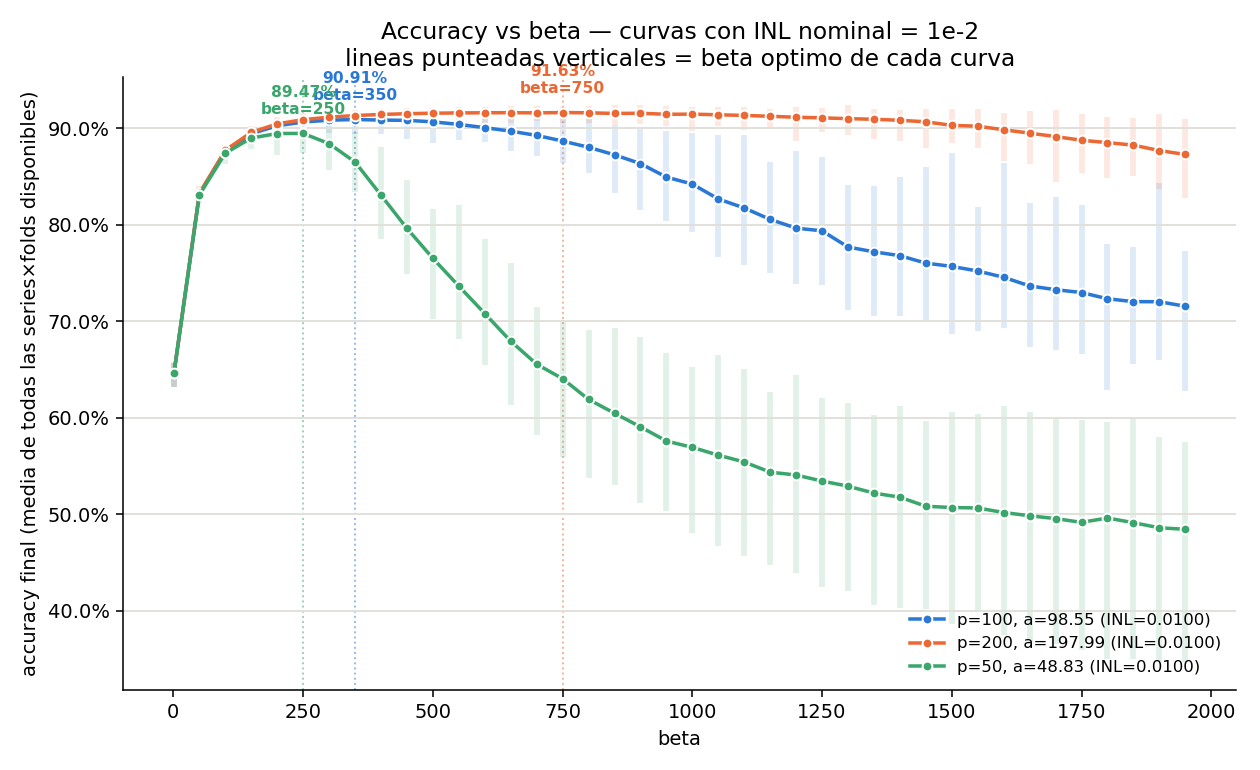
\includegraphics[width=\linewidth]{../data_beta_grid_search_SP/resumen_por_INL/accuracy_vs_beta_INL_1e-2.png}
\end{minipage}\hfill
\begin{minipage}{0.49\textwidth}
\centering
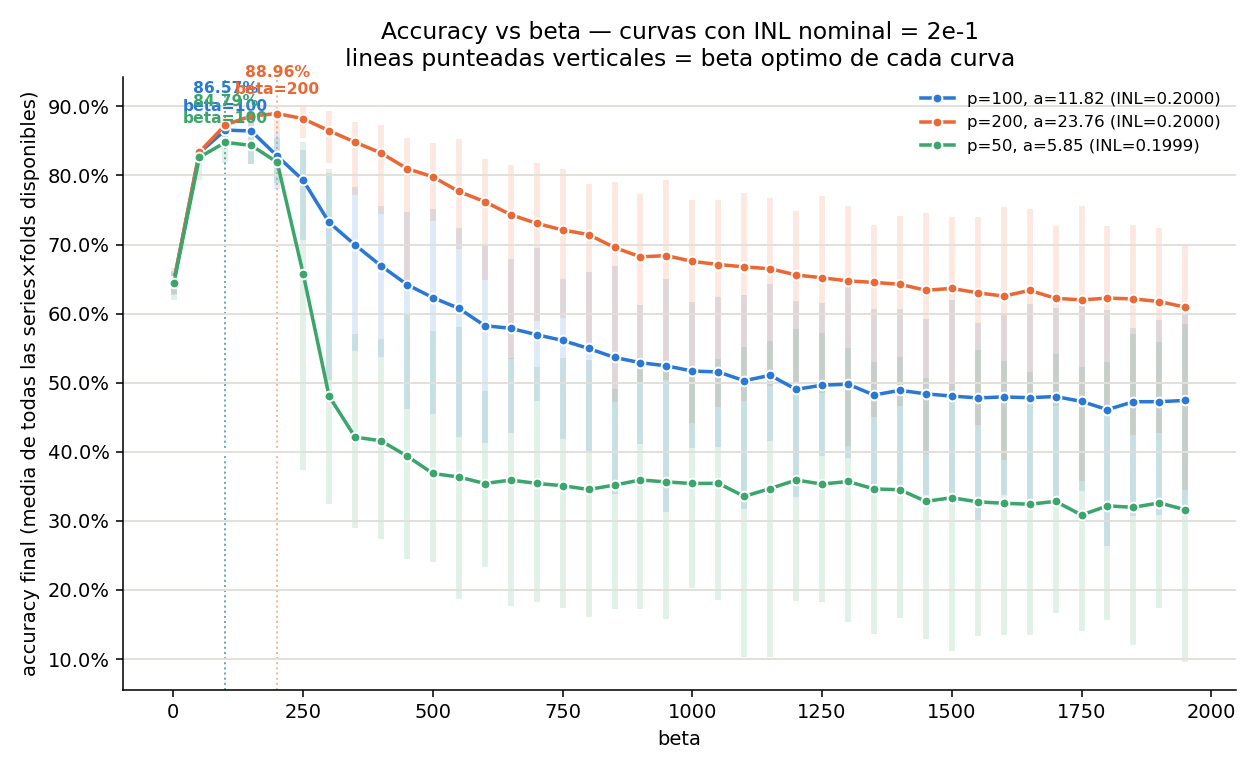
\includegraphics[width=\linewidth]{../data_beta_grid_search_SP/resumen_por_INL/accuracy_vs_beta_INL_2e-1.png}
\end{minipage}
\caption{Accuracy final vs.\ $\beta$ para las curvas con INL nominal
\texttt{1e-2} (izq.) y \texttt{2e-1} (der.). Figuras ya generadas por el
proyecto (\texttt{plot\_accuracy\_vs\_beta\_por\_INL.py}), no regeneradas en
este reporte. El caso \texttt{INL=1e-2, p=200} es casi una meseta entre
$\beta\approx150$ y $\beta\approx1000$ (91--92\% de accuracy): su
``óptimo'' puntual es más sensible al ruido y a la resolución de la grilla
(paso 50) que el resto.}
\end{figure}

\section{Método}

Script nuevo: \texttt{validar\_beta\_optimo.py} (el único código nuevo de
este reporte). Para cada una de las 6 curvas:
\begin{enumerate}
\item Lee \texttt{pulsos\_pot}, \texttt{a\_pot}, $G_{\min}$, $G_{\max}$,
  concavidad del \texttt{config\_*.json} real de esa corrida (no se
  transcriben números a mano).
\item Genera \texttt{pot}, \texttt{dep} con
  \texttt{generar\_curvas\_pot\_dep(...)} --- función ya provista en
  \texttt{MemCrossbarClass\_beta\_por\_capa.py}, importada sin modificar.
\item Estima $\sigma_W$ por Monte Carlo: una única llamada a
  \texttt{G0\_initialization('random', pot, dep, D\_in=20000, D\_out=10)}
  (función ya provista) y calcula $\mathrm{std}(G[{:},0{::}2]-G[{:},1{::}2])$.
  $D_{\mathrm{in}}=20000$ es solo para tener una muestra grande y estable de
  $\sigma_W$; no representa el tamaño real de la crossbar ($N=784$ se usa
  aparte, en la fórmula).
\item Calcula $V_{\mathrm{rms}}$ sobre \texttt{X\_train\_mnist.npy} (el
  mismo dataset del grid search).
\item Compara contra \texttt{beta\_optimo} empírico de
  \texttt{resumen\_optimos.csv}.
\end{enumerate}
Ningún entrenamiento de red se ejecuta en este script; solo estadística
sobre funciones y datos ya provistos.

\section{Resultados}

\begin{table}[htbp]
\centering
\small
\begin{tabular}{@{}llrrrrrr@{}}
\toprule
INL nominal & $p$ & $a$ & $\sigma_W$ (S) & $\beta_{\mathrm{pred}}$ ($\kappa{=}1$) & $\beta_{\text{óptimo}}$ emp. & acc.\ óptima & $\kappa$ implicado \\
\midrule
1e-2 & 50  & 48.83  & 3.789e-04 & 281.7 & \textbf{250} & 89.47\% & 0.89 \\
1e-2 & 100 & 98.55  & 3.790e-04 & 281.6 & \textbf{350} & 90.91\% & 1.24 \\
1e-2 & 200 & 197.99 & 3.796e-04 & 281.1 & \textbf{750} & 91.63\% & 2.67 \\
2e-1 & 50  & 5.85   & 5.570e-04 & 191.6 & \textbf{100} & 84.79\% & 0.52 \\
2e-1 & 100 & 11.82  & 5.563e-04 & 191.9 & \textbf{100} & 86.57\% & 0.52 \\
2e-1 & 200 & 23.76  & 5.565e-04 & 191.8 & \textbf{200} & 88.96\% & 1.04 \\
\bottomrule
\end{tabular}
\caption{$V_{\mathrm{rms}}(\texttt{X\_train\_mnist.npy})=0.33467$, $N=784$
en las 6 filas. $\kappa$ implicado $=\beta_{\text{óptimo,emp}}\cdot\sqrt{N}\cdot\sigma_W\cdot V_{\mathrm{rms}}$.}
\end{table}

\textbf{$\kappa$ implicado} (media geométrica): $\mathbf{0.97}$ --- dentro
del rango $O(1$--$10)$ que predice el argumento de LeCun/Prezioso --- pero
con un rango $[0.52,\,2.67]$ (cociente máx/mín $=5.1$). Ajuste log-log
$\beta_{\text{óptimo}} \sim (1/(\sqrt{N}\sigma_W V_{\mathrm{rms}}))^{\text{slope}}$
sobre las 6 filas: $\text{slope}=3.0$ (teoría: 1), $R^2=0.68$ --- dominado
por el hecho de que $\sigma_W$ casi no cambia entre $p=50,100,200$ de un
mismo INL nominal (por diseño: $a$ se ajustó para eso) mientras que
$\beta_{\text{óptimo}}$ sí cambia mucho.

\begin{figure}[htbp]
\centering
\begin{minipage}{0.49\textwidth}
\centering
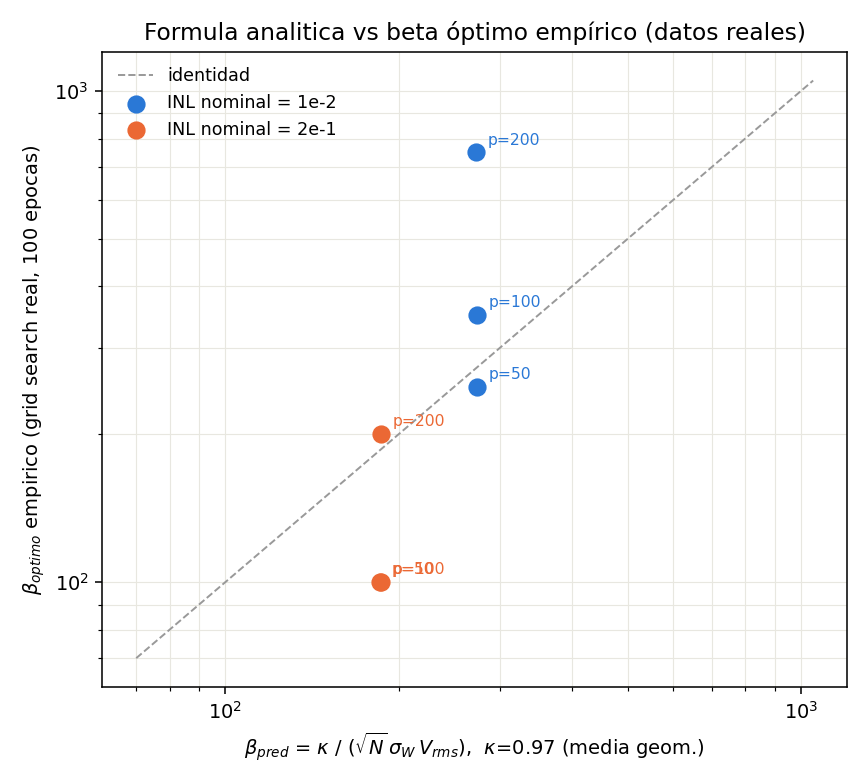
\includegraphics[width=\linewidth]{beta_pred_vs_empirico.png}
\end{minipage}\hfill
\begin{minipage}{0.49\textwidth}
\centering
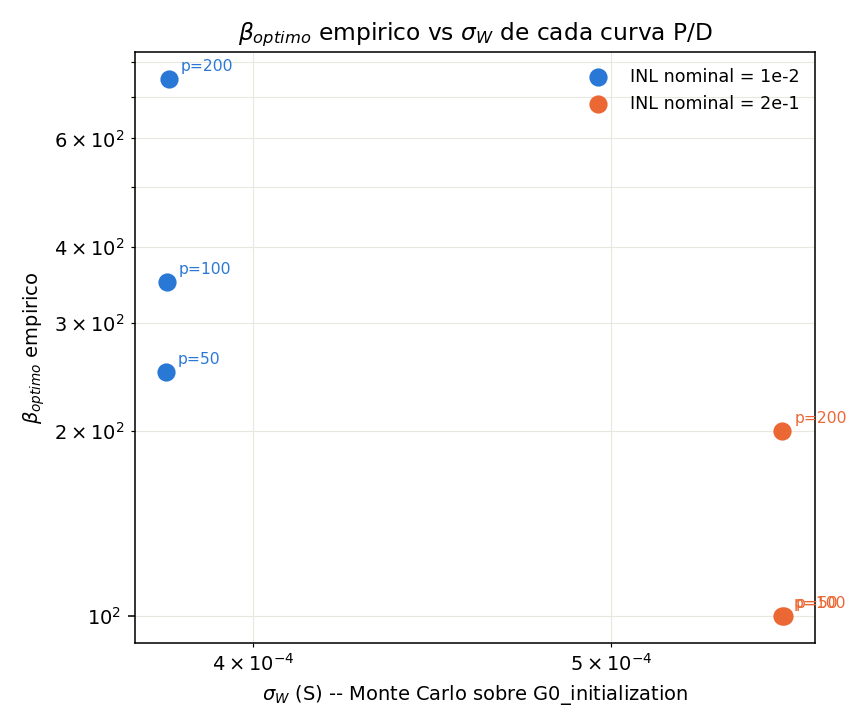
\includegraphics[width=\linewidth]{beta_pred_vs_sigmaW.png}
\end{minipage}
\caption{Izquierda: $\beta$ predicho por la fórmula (con $\kappa$=media
geométrica) vs.\ $\beta$ óptimo empírico, escala log-log, línea punteada =
identidad. Derecha: $\beta$ óptimo empírico vs.\ $\sigma_W$ de cada curva
P/D --- a $\sigma_W$ casi fijo dentro de un INL, $\beta_{\text{óptimo}}$
varía igual mucho con $p$.}
\end{figure}

\subsection{Lo que la fórmula (*) SÍ predice bien}
\begin{itemize}
\item \textbf{Orden de magnitud}: $\kappa\approx1$ en las 6 curvas,
  consistente con la recomendación de LeCun/Prezioso ($O(1$--$10)$) y con la
  verificación externa ya hecha en el reporte analítico previo contra el
  hardware real de Prezioso et al.\ ($\kappa\approx3$, mismo orden).
\item \textbf{Dirección entre ventanas de no linealidad distintas}: el
  grupo \texttt{INL=2e-1} tiene $\sigma_W$ más grande (0.557~mS vs.\
  0.379~mS) y, en las 6 filas, $\beta_{\text{óptimo}}$ es sistemáticamente
  más chico en ese grupo (100--200 frente a 250--750) --- la misma
  dirección que predice (*) y que ya había encontrado el reporte previo
  (Barrido C) con una búsqueda reducida.
\end{itemize}

\subsection{Lo que la fórmula (*) NO predice}

\textbf{Dependencia con el número de pulsos a INL fijo.} Dentro de un mismo
INL nominal, $a_{\mathrm{pot}}$ se ajusta junto con $p$ para mantener
$\sigma_W$ casi constante (variación $<1\%$ entre $p=50,100,200$), así que
(*) predice prácticamente el mismo $\beta_{\text{óptimo}}$ para los tres.
La red entrenada completa dice lo contrario: $\beta_{\text{óptimo}}$
\textbf{crece con $p$} en ambos INL ($250\to350\to750$ y $100\to100\to200$).
Esto reproduce, ahora con entrenamiento convergido (100 épocas) en vez de 1
época, el mismo resultado negativo que ya había anticipado
\texttt{Reporte\_beta\_optimo\_analitico.pdf} (Sección 4.3 y Sección 5,
punto 7): $\sigma_W$ describe la distribución estática agrupada de
conductancias en la inicialización, pero no la resolución/paso de la regla
de Manhattan (cuántos niveles de conductancia hay entre $G_{\min}$ y
$G_{\max}$), que sí depende fuertemente de $p$.

\subsection{Diagnóstico exploratorio: paso medio de la curva P/D}

Como chequeo de la sugerencia del propio reporte previo (Sec.\ 5, punto 7:
``un descriptor relacionado con la pendiente local de la curva P/D, no solo
$\sigma_W$''), el script también calcula, sin agregar ningún método nuevo,
$\text{paso\_medio}=\mathrm{mean}(|\mathrm{pot}[i{+}1]-\mathrm{pot}[i]|)$ de
la curva ya generada por \texttt{generar\_curvas\_pot\_dep}, y el $\kappa_2$
implicado al reemplazar $\sigma_W$ por ese paso medio en (*):

\begin{table}[htbp]
\centering
\small
\begin{tabular}{@{}llrr@{}}
\toprule
carpeta & INL & paso\_medio\_pot (S) & $\kappa_2$ implicado \\
\midrule
$p=50$  & 1e-2 & 1.815e-05 & 0.0425 \\
$p=100$ & 1e-2 & 9.038e-06 & 0.0296 \\
$p=200$ & 1e-2 & 4.509e-06 & 0.0317 \\
$p=50$  & 2e-1 & 1.837e-05 & 0.0172 \\
$p=100$ & 2e-1 & 9.091e-06 & 0.0085 \\
$p=200$ & 2e-1 & 4.523e-06 & 0.0085 \\
\bottomrule
\end{tabular}
\end{table}

Dentro de cada INL, $p=100$ y $p=200$ quedan muy consistentes entre sí
($\kappa_2$ difiere menos del 7\%) --- mucho mejor que con $\sigma_W$ ---
pero $p=50$ sigue siendo un valor atípico en ambos grupos (${\sim}1.4\times$--$2\times$
más alto), y el $\kappa_2$ no es la misma constante entre los dos INL
(difiere $\times3.5$, mientras que con $\sigma_W$ la dirección entre INL sí
se explica). Es decir: \textbf{ningún descriptor único explica ambos ejes a
la vez} (INL/ventana de conductancia por un lado, número de pulsos por el
otro) con las 6 curvas disponibles. Esto es exactamente el resultado
``mixto'' que el reporte previo ya anticipaba, ahora confirmado con
entrenamiento real convergido en vez de una búsqueda reducida de 1 época.
Nótese además que $p=50$ es, en ambos INL, el caso con el pico de accuracy
más chato/inestable en la figura de accuracy-vs-$\beta$ (Sección 3), lo que
puede inflar el ruido de su $\beta_{\text{óptimo}}$ puntual además del
efecto físico.

\section{Conclusiones}

\begin{enumerate}
\item La fórmula (*) da el \textbf{orden de magnitud correcto} de
  $\beta_{\text{óptimo}}$ ($\kappa$ implicado $\approx1$, dentro de
  $O(1$--$10)$) en las 6 configuraciones reales validadas aquí, con
  entrenamiento \textbf{completo} (100 épocas) --- no solo en la búsqueda
  reducida del reporte previo ni en el chequeo externo contra Prezioso et
  al.
\item \textbf{Predice correctamente la dirección} del efecto de la ventana
  de conductancia/no linealidad global ($\sigma_W$ más grande $\Rightarrow$
  $\beta_{\text{óptimo}}$ más chico) entre los dos grupos de INL nominal.
\item \textbf{No predice} el efecto, igual de grande, del número de pulsos
  de la curva P/D a INL nominal fijo: $\beta_{\text{óptimo}}$ sube
  claramente con $p$ mientras $\sigma_W$ se mantiene ${\sim}$constante por
  diseño del experimento. Reemplazar $\sigma_W$ por el paso medio de la
  curva mejora la consistencia dentro de un mismo INL (salvo $p=50$) pero
  rompe la consistencia entre INL --- ningún descriptor único usado aquí
  captura los dos efectos a la vez.
\item \textbf{Recomendación práctica} (igual que ya sugería el reporte
  previo): (*) sirve como estimador inicial de orden de magnitud para
  acotar el rango de \texttt{search\_best\_beta} (por ejemplo,
  $\beta\in[\beta_{\mathrm{pred}}/3,\ \beta_{\mathrm{pred}}\cdot10]$ con
  $\kappa\approx1$--$3$) y ahorrar cómputo de grilla, pero \textbf{no
  reemplaza} la búsqueda por grid-search+K-fold para fijar el valor final:
  la propia variación de $\kappa$ (factor $5\times$ entre las 6 curvas)
  indica que el resultado de (*) por sí solo no es preciso.
\item Esta validación usa 6 puntos con $N=784$ fijo (no vuelve a poner a
  prueba la dependencia con el tamaño de la crossbar, ya explorada --- con
  una búsqueda reducida --- en el Barrido A del reporte previo). Sería
  valioso repetir este mismo procedimiento de validación, con datos de
  entrenamiento completo como los de \texttt{data\_beta\_grid\_search\_SP/},
  para un barrido de $N$ y de arquitectura MLP ($\beta$ por capa), cuando
  existan esos datos.
\end{enumerate}

\section{Registro de códigos usados}
\label{sec:registro}

Nada de lo siguiente fue modificado; se usó tal cual está en el
repositorio.

\begin{itemize}
\item \textbf{\texttt{validar\_beta\_optimo.py}} --- Único script nuevo.
  Calcula $\sigma_W$ (Monte Carlo), $V_{\mathrm{rms}}$, $\beta_{\mathrm{pred}}$
  y compara con \texttt{resumen\_optimos.csv}. Genera
  \texttt{resultados\_validacion\_beta\_optimo.csv},
  \texttt{beta\_pred\_vs\_empirico.png}, \texttt{beta\_pred\_vs\_sigmaW.png}.
\item \texttt{MemCrossbarClass\_beta\_por\_capa.py}
  $\to$ \texttt{generar\_curvas\_pot\_dep()} --- Genera las curvas
  \texttt{pot}/\texttt{dep} reales de cada configuración (mismos parámetros
  que el grid search).
\item \texttt{MemCrossbarClass\_beta\_por\_capa.py}
  $\to$ \texttt{G0\_initialization('random', ...)} --- Muestreo Monte Carlo
  de $W=G^+-G^-$ para estimar $\sigma_W$.
\item \texttt{Crossbar\_train\_experimento\_beta\_por\_capa.py} --- No se
  ejecutó; se usó solo para confirmar parámetros fijos del grid search
  ($N=784$, $G_{\min}/G_{\max}$, dataset, arquitectura SP) y el significado
  de los campos de los \texttt{config\_*.json}.
\item \texttt{data\_beta\_grid\_search\_SP/plot\_accuracy\_vs\_beta\_por\_INL.py}
  --- No se ejecutó en esta sesión; ya había generado
  \texttt{resumen\_por\_INL/resumen\_optimos.csv} y las figuras
  \texttt{accuracy\_vs\_beta\_INL\_*.png} usadas como fuente de verdad
  empírica y como contexto de forma de los picos (Sección 3).
\item \texttt{data\_beta\_grid\_search\_SP/analizar\_distribucion\_por\_INL.py}
  --- No se ejecutó; mencionado solo como el script que generó las figuras
  de dispersión/asimetría de \texttt{resumen\_por\_INL/} (no usadas
  directamente en este reporte).
\item \texttt{data\_beta\_grid\_search\_SP/beta\_grid\_search\_SP\_INL\_*/config\_*.json}
  --- Fuente de los parámetros reales (\texttt{pulsos\_pot},
  \texttt{a\_pot}, $G_{\min}$, $G_{\max}$, concavidad) de cada una de las 6
  curvas.
\item \texttt{X\_train\_mnist.npy} --- Dataset real usado para calcular
  $V_{\mathrm{rms}}$ (idéntico al usado en el grid search).
\item \texttt{papers/Reporte\_beta\_optimo\_analitico.pdf} --- Fuente de la
  fórmula (*) validada aquí y de la sugerencia de diagnóstico (paso medio,
  Sección 5.3).
\end{itemize}

Archivos generados por este reporte (todos en
\texttt{validacion\_formula\_beta\_optimo/}): \texttt{validar\_beta\_optimo.py},
\texttt{resultados\_validacion\_beta\_optimo.csv},
\texttt{beta\_pred\_vs\_empirico.png}, \texttt{beta\_pred\_vs\_sigmaW.png},
\texttt{reporte\_validacion\_beta\_optimo.tex} y este PDF.

\end{document}
